\documentclass{beamer}

\usepackage[utf8]{inputenc}
\usepackage{amssymb, amsfonts, latexsym, amsthm, amsmath, framed}
\usepackage{esvect}
\usepackage{parskip}

\usepackage{amsmath, amssymb, framed, tcolorbox}
\tcbuselibrary{theorems}

\usepackage{mathrsfs}
% \usepackage[hidelinks,colorlinks=true,linkcolor=blue,citecolor=blue]{hyperref}

\usepackage{xcolor}

\usepackage{natbib}
\bibliographystyle{plainnat}

\newcommand{\ba}{\backslash}
\newcommand{\Q}{\mathbb{Q}}
\newcommand{\C}{\mathbb{C}}
\newcommand{\R}{\mathbb{R}}
\newcommand{\N}{\mathbb{N}}
\newcommand{\Z}{\mathbb{Z}}
\newcommand{\F}{\mathbb{F}}
\newcommand{\rank}{\text{rank}}

\newcounter{mytheorem}[section] \def\themytheorem{\thesection.\arabic{mytheorem}}

\definecolor{myteal}{cmyk}{0.5,0,0.15,0}
\usecolortheme[named=myteal]{structure}

\definecolor{my-yellow}{cmyk}{0,0.2,0.7,0,1.00}
\definecolor{my-blue}{cmyk}{0.80, 0.13, 0.14, 0.04, 1.00}
\definecolor{my-green}{cmyk}{0.4,0,0.4,0,1.00}
\tcbset{
defstyle/.style={fonttitle=\bfseries\upshape, colback=my-yellow!5,colframe=my-yellow!80!black},
theostyle/.style={fonttitle=\bfseries\upshape, colback=my-blue!5,colframe=my-blue!80!black},
corstyle/.style={fonttitle=\bfseries\upshape, colback=my-green!5,colframe=my-green!80!black},
}

\tcbmaketheorem{defn}{Definition}{theostyle}{mytheorem}{def}
\tcbmaketheorem{theom}{Theorem}{theostyle}{mytheorem}{theo}
\tcbmaketheorem{coro}{Corollary}{corstyle}{mytheorem}{cor}
\tcbmaketheorem{exm}{Example}{corstyle}{mytheorem}{eg}


\usetheme{Madrid}


\title{Lie algebra, $\mathfrak{sl}_3$ and representation}
\subtitle{MATH 334 Term Paper Presentation}
\date{Apr 25, 2022}
\author{Yuxuan Sun}
\institute{Haverford College}

\begin{document}
	
\begin{frame}
\titlepage
\end{frame}

\section{first}

\begin{frame}{Lie algebra}

	\begin{defn}{bracket, commutator, and Lie algebra}{defn:bracket}
	A vector space $L$ over a field $F$, with an operation $\left[ \cdot, \cdot \right] $ from $L \times L \to  L$, called the  \textbf{bracket} or \textbf{commutator} of $x$ and  $y$, is called a  \textbf{Lie algebra} over $F$ if the following axioms are satisfied:
\begin{enumerate}
		 \item The bracket operation is bilinear
\begin{enumerate}
	\item $[x,y_1+y_2] = [x,y_1] + [x,y_2]$ and $[x_1+x_2,y] = [x_1,y] + [x_2,y]$
	\item $[\lambda x, y] = \lambda[x,y] = [x, \lambda y]$
\end{enumerate}
		 \item $[x,x] = 0$
		 \item $[x,[y,z]]+[y,[z,x]] +[z,[x,y]] = 0$
	\end{enumerate}
\end{defn}
\begin{theom}{anti-commutativity of Lie algebra}{}
		\[
			[x,y] = -[y,x]
		\] 
\end{theom}	

\end{frame}

\begin{frame}{Lie algebra}
	\begin{exm}{$\mathfrak{sl}_2(\R)$}{}
		$\mathfrak{sl}_2(\R)$ is a set of  $2 \times 2$ matrices with trace  $0$, in other words:
	\[
		\mathfrak{sl}_2(\R) = \left\{ \begin{bmatrix} a & b \\ c & -a \end{bmatrix} \mid a,b,c \in \R  \right\} 
	\] equipped with bracket $[A,B] = AB - BA$.
\end{exm}
\end{frame}

\begin{frame}{Lie algebra}
	\begin{exm}{$\mathfrak{sl}_2(\R)$}{}
		$\mathfrak{sl}_2(\R)$ is a set of  $2 \times 2$ matrices with trace  $0$, in other words:
	\[
		\mathfrak{sl}_2(\R) = \left\{ \begin{bmatrix} a & b \\ c & -a \end{bmatrix} \mid a,b,c \in \R  \right\} 
	\] equipped with bracket $[A,B] = AB - BA$.
\tcblower
we could come up with a basis for this $3$-dimensional vector space:  \[
	\mathcal{B}_{\mathfrak{sl}_2} = \left\{ H = \begin{bmatrix} 1 & 0 \\ 0 &-1 \end{bmatrix}, X =\begin{bmatrix} 0 & 1 \\ 0 &0 \end{bmatrix}, Y = \begin{bmatrix} 0 & 0 \\ 1 &0 \end{bmatrix} \right\} 
\] 
\end{exm}
\end{frame}


\begin{frame}{Lie algebra}
Let's increase our dimension a bit.

\begin{exm}{$\mathfrak{sl}_3(\R)$}{}
	$\mathfrak{sl}_{3}$ is a set of $3 \times 3$ matrices with trace 0, in other words:  \[
		\mathfrak{sl}_{3} = \left\{ \begin{bmatrix} a & c & d \\
		e & -a+b & f \\ g & h & -b\end{bmatrix} \mid a,b,c,d,e,f,g,h \in \R \right\} 
	\] 
\end{exm}

\end{frame}


\addtocounter{mytheorem}{-1}
\begin{frame}{Lie algebra}
Let's increase our dimension a bit.

\begin{exm}{$\mathfrak{sl}_3(\R)$}{}
	$\mathfrak{sl}_{3}$ is a set of $3 \times 3$ matrices with trace 0, in other words:  \[
		\mathfrak{sl}_{3}(\R) = \left\{ \begin{bmatrix} a & c & d \\
		e & -a+b & f \\ g & h & -b\end{bmatrix} \mid a,b,c,d,e,f,g,h \in \R \right\} 
	\] 
\tcblower
similarly, the basis is: \[
	\mathcal{B}_{\mathfrak{sl}_{3}} = \left\{ H_1 = \begin{bmatrix} 1 & 0 &0 \\ 0 & -1 & 0 \\ 0 &0 &0 \end{bmatrix}, H_2 = \begin{bmatrix} 0 &0 &0 \\ 0 &1&0 \\ 0&0&-1 \end{bmatrix}   \right\} \bigcup \left\{ E_{i,j} \mid i \neq j\right\}. 
\] $E_{i,j}$ is a matrix where ${E_{i,j}}_{ij} = 1$ and other places are $0$.
\end{exm}

\end{frame}


\begin{frame}{some linear algebra}
	\begin{defn}{subspace $\mathfrak{h} \subseteq \mathfrak{sl}_3(\R)$}{}
		Let  $\mathfrak{h}$ be the two-dimensional subspace of all diagonal matrices, namely:  \[
			\mathfrak{h} = \text{span}{\left\{ H_1 = \begin{bmatrix} 1 & 0 &0 \\ 0 & -1 & 0 \\ 0 &0 &0 \end{bmatrix}, H_2 = \begin{bmatrix} 0 &0 &0 \\ 0 &1&0 \\ 0&0&-1 \end{bmatrix}   \right\} }
		\] 
	\end{defn}
\end{frame}

\begin{frame}{some linear algebra}
	\begin{defn}{subspace $\mathfrak{h} \subseteq \mathfrak{sl}_3(\R)$}{}
		Let  $\mathfrak{h}$ be the two-dimensional subspace of all diagonal matrices, namely:  \[
			\mathfrak{h} = \text{span}{\left\{ H_1 = \begin{bmatrix} 1 & 0 &0 \\ 0 & -1 & 0 \\ 0 &0 &0 \end{bmatrix}, H_2 = \begin{bmatrix} 0 &0 &0 \\ 0 &1&0 \\ 0&0&-1 \end{bmatrix}   \right\} }
		\] 
	\end{defn}
	What does it mean to be an eigenspace for $\mathfrak{h}$?
\end{frame}

\begin{frame}{some linear algebra}
	Let's pick an arbitrary $H \in \mathfrak{h}$ and $M \in \mathfrak{sl}_3(\R)$, namely: \[
		H = \def\a{\color{red}a} \begin{bmatrix} \a_1 & 0 & 0 \\ 0 & \a_2 &0 \\ 0 &0 &\a_3 \end{bmatrix}, M = \def\m{\color{blue}m} \begin{bmatrix} \m_{11} & \m_{12} & \m_{13} \\ \m_{21} & \m_{22} & \m_{23} \\ \m_{31} & \m_{32} & \m_{33} \end{bmatrix} 
	\] 
\end{frame}


\begin{frame}{some linear algebra}
	Let's pick an arbitrary $H \in \mathfrak{h}$ and $M \in \mathfrak{sl}_3(\R)$, namely: \[
		H = \def\a{\color{red}a} \begin{bmatrix} \a_1 & 0 & 0 \\ 0 & \a_2 &0 \\ 0 &0 &\a_3 \end{bmatrix}, M = \def\m{\color{blue}m} \begin{bmatrix} \m_{11} & \m_{12} & \m_{13} \\ \m_{21} & \m_{22} & \m_{23} \\ \m_{31} & \m_{32} & \m_{33} \end{bmatrix} 
	\]
	Let's see the result under bracket, i.e. $[H,M] = ?$
\end{frame}


\begin{frame}{some linear algebra}
	Let's pick an arbitrary $H \in \mathfrak{h}$ and $M \in \mathfrak{sl}_3(\R)$, namely: \[
		H = \def\a{\color{red}a} \begin{bmatrix} \a_1 & 0 & 0 \\ 0 & \a_2 &0 \\ 0 &0 &\a_3 \end{bmatrix}, M = \def\m{\color{blue}m} \begin{bmatrix} \m_{11} & \m_{12} & \m_{13} \\ \m_{21} & \m_{22} & \m_{23} \\ \m_{31} & \m_{32} & \m_{33} \end{bmatrix} 
	\]
	Let's see the result under bracket, i.e. $[H,M] = ?$
	\begin{align*}
		[D,M] &= \def\a{\color{red}a} \def\m{\color{blue}m} \begin{bmatrix} (\a_1-\a_1)\m_{11} & (\a_1-\a_2)\m_{12} & (\a_1-\a_3)\m_{13} \\ (\a_2-\a_1)\m_{21} & (\a_2-\a_2)\m_{22} & (\a_2-\a_3)\m_{23} \\ (\a_3-\a_1)\m_{31} & (\a_3-\a_2)\m_{32} & (\a_3-\a_3)\m_{33} \end{bmatrix} \\
		      &=  \def\a{\color{red}a} \def\m{\color{blue}m} \begin{bmatrix} 0 \cdot \m_{11} & (\a_1-\a_2)\m_{12} & (\a_1-\a_3)\m_{13} \\ (\a_2-\a_1)\m_{21} & 0 \cdot \m_{22} & (\a_2-\a_3)\m_{23} \\ (\a_3-\a_1)\m_{31} & (\a_3-\a_2)\m_{32} & 0 \cdot \m_{33} \end{bmatrix} 
	\end{align*}
\end{frame}

\begin{frame}{some linear algebra}
	\[ [H,M] = \def\a{\color{red}a} \def\m{\color{blue}m} \begin{bmatrix} 0& (\a_1-\a_2)\m_{12} & (\a_1-\a_3)\m_{13} \\ (\a_2-\a_1)\m_{21} & 0& (\a_2-\a_3)\m_{23} \\ (\a_3-\a_1)\m_{31} & (\a_3-\a_2)\m_{32} & 0 \end{bmatrix} \] 
	\def\a{\color{red}a}
	observation: for $M$ to be an eigenvector under bracket  $H$, i.e.  $[H,M] = \lambda M$ for some  $\lambda$,  $M$ must be all  $0$ on the diagonal and only one place not equal to  $0$. 

%	For the second part, don't forget we have a constrain: $\a_1+\a_2+\a_3 = 0$ 

%	if, for example, $\lambda(\a_1-\a_3) = \lambda(\a_2-\a_3)$, we'll have $\a_1=\a_2$
\end{frame}


\begin{frame}{linear functional}	
	\[ [H,M] = \def\a{\color{red}a} \def\m{\color{blue}m} \begin{bmatrix} 0& (\a_1-\a_2)\m_{12} & (\a_1-\a_3)\m_{13} \\ (\a_2-\a_1)\m_{21} & 0& (\a_2-\a_3)\m_{23} \\ (\a_3-\a_1)\m_{31} & (\a_3-\a_2)\m_{32} & 0 \end{bmatrix} \]

	one could see we have potentially $6$ eigenvalues for each  $H \in \mathfrak{h}$: $a_1-a_2, a_1-a_3, a_2-a_3, a_2-a_1, a_3-a_1, a_3-a_2$. 
	% Since we are asking for the eigenspace of $\mathfrak{h}$, we need a way to get  $a_i-a_j$ from any  $H \in \mathfrak{h}$ for us, thus we could define a linear functional:

	\begin{defn}{$L_i$}{}
	$L_i$ is a linear functional s.t. \[
		L_i \begin{bmatrix} a_1 & 0 &0 \\ 0 & a_2 & 0 \\ 0 &0 &a_3 \end{bmatrix} = a_i 
	\] it satisfies the requirement of a linear functional: 

	$L_i(A+B) = L_i(A) + L_i(B), L_i(aA) = aL_i(A)$.
	\end{defn}
\end{frame}

\begin{frame}{eigenvalues and eigenspaces}
	in other words, the set of all eigenvalues of $\mathfrak{h}$ is  \[
		\mathfrak{h}^* = \R \left\{ L_1,L_2,L_3 \right\} / (L_1+L_2+L_3=0). 
	\] given any finite-dimensional representationl $V$ of  $\mathfrak{sl}_3(\R)$, the eigenspace associated to the eigenvalue $\alpha \in \mathfrak{h}$ is the subspace of all vectors $v \in V$ s.t. \[
	H(v) = \alpha(H) \cdot v
\] for all $H \in \mathfrak{h}$.
\end{frame}

\begin{frame}{representation and action}
	What's $H(v)$?
\end{frame}

\section{representation}

\begin{frame}{representation and action}
	
	\begin{defn}{adjoint representation of $\mathfrak{sl}_3(\R)$}{}
		Give $X \in \mathfrak{sl}_3(\R)$, define a linear map $ad_X : \mathfrak{sl}_3(\R) \to \mathfrak{sl}_3(\R)$ as: \[
			ad_X(Y) = [X,Y]
		\] the map $X \mapsto ad_X$ is called an adjoint representation of $\mathfrak{sl}_3(\R)$.
	\end{defn}
\end{frame}

\begin{frame}{representation and action}
	What's $H(v)$?
	
	\begin{defn}{adjoint representation of $\mathfrak{sl}_3(\R)$}{}
		Give $X \in \mathfrak{sl}_3(\R)$, define a linear map $ad_X : \mathfrak{sl}_3(\R) \to \mathfrak{sl}_3(\R)$ as: \[
			ad_X(Y) = [X,Y]
		\] the map $X \mapsto ad_X$ is called an adjoint representation of $\mathfrak{sl}_3(\R)$.
	\end{defn}
	so if our $V$ is the adjoint representation, given an eigenvalue  $\alpha \in \mathfrak{h}^*$ and $v \in V$, we'll have \[
		H(v) = ad_H(v) = [H, v] = \alpha(H) \cdot v
	\] 
\end{frame}

\begin{frame}{representation and action}
	Recall 
	\[ [H,M] = \def\a{\color{red}a} \def\m{\color{blue}m} \begin{bmatrix} 0& (\a_1-\a_2)\m_{12} & (\a_1-\a_3)\m_{13} \\ (\a_2-\a_1)\m_{21} & 0& (\a_2-\a_3)\m_{23} \\ (\a_3-\a_1)\m_{31} & (\a_3-\a_2)\m_{32} & 0 \end{bmatrix} \]
	we could see that for each eigenvalue $\alpha \in \mathfrak{h}^*$, i.e. $L_i - L_j$ (so basically $a_i-a_j$), the eigenspace is generated by the other basis element  $E_{i,j}$ where $i \neq j$ and $E_{i,j}$ has all but one entry $ij$ zero, for example:  \[
		E_{1,3} = \begin{bmatrix} 0 & 0 & 1 \\ 0 & 0 &0 \\ 0 &0 &0 \end{bmatrix} 
	\] 
\end{frame}

\begin{frame}{why?}
	Notice that for the adjoint representation of $\mathfrak{sl}_3(\R)$, we have the following decomposition:  \[
		\mathfrak{sl}_3(\R) = \mathfrak{h} \oplus \left( \oplus V_\alpha \right) 
	\] where $\alpha$ ranges over $\mathfrak{h}^*$ and $V_{\alpha}$ is the eigenspace w.r.t $\alpha$
\end{frame}

\begin{frame}{why?}
	Notice that for the adjoint representation of $\mathfrak{sl}_3(\R)$, we have the following decomposition:  \[
		\mathfrak{sl}_3(\R) = \mathfrak{h} \oplus \left( \oplus V_\alpha \right) 
	\] where $\alpha$ ranges over $\mathfrak{h}^*$ and $V_{\alpha}$ is the eigenspace w.r.t $\alpha$

	this is a psecial case of a general statement:
	\begin{theom}{}{}
		For any semisimple Lie algebra $\mathfrak{g}$ (it is a direct sum of simple Lie algebras (non-abelian Lie algebras without any non-zero proper ideals), we could find an abelian subalgebra(closed under bracket)  $\mathfrak{h} \subset \mathfrak{g}$ s.t. the action of $\mathfrak{h}$ on any representation $V$ could be written as a direct sum decomposition of $V$ into eigenspaces  $V_{\alpha}$ for $\mathfrak{h}$.
	\end{theom}
\end{frame}

\begin{frame}{graph of eigenspaces}
\begin{center} 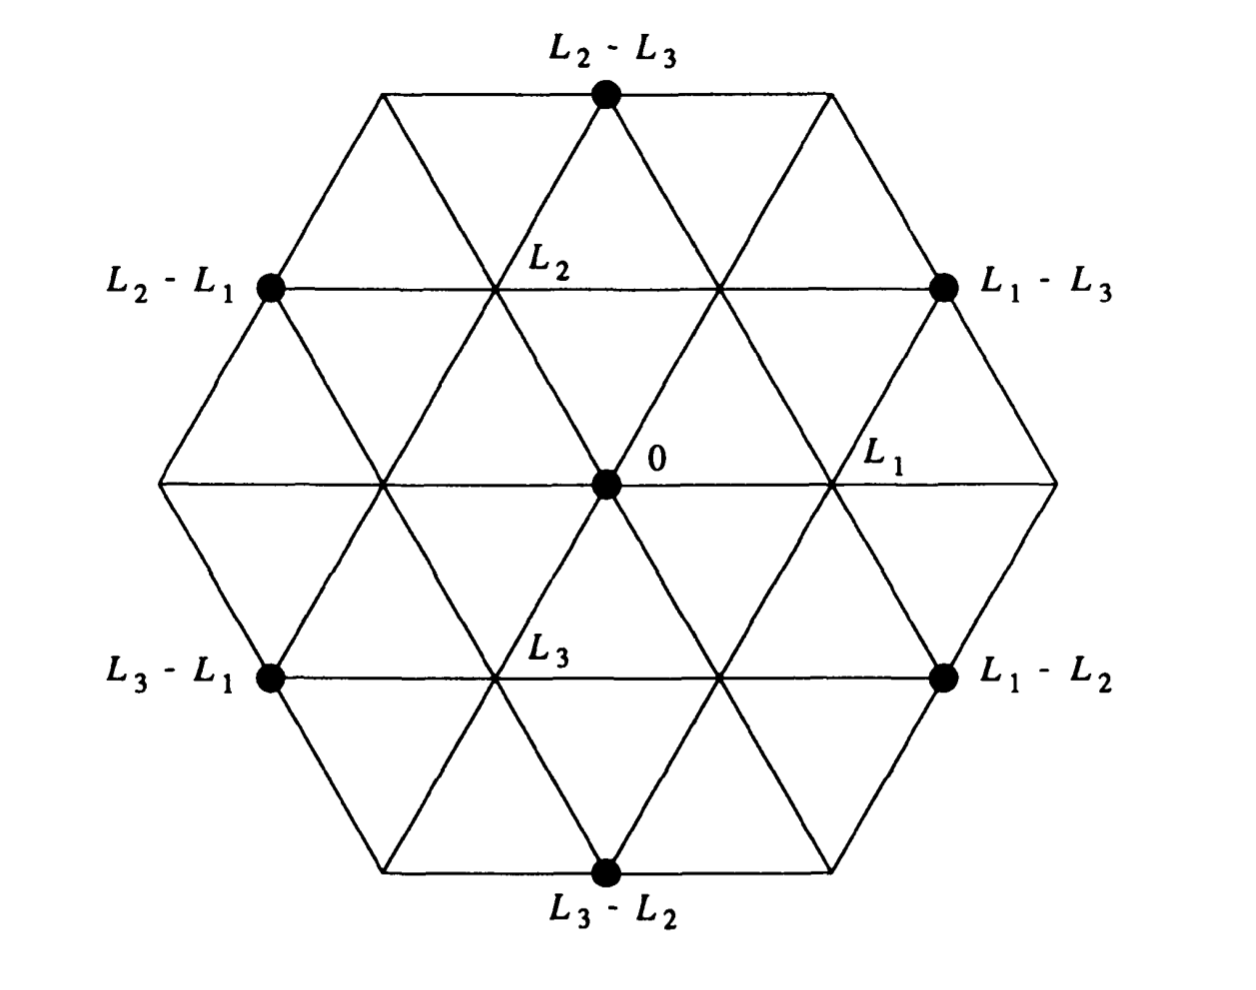
\includegraphics[scale=.3]{eigenvalue.jpg}\end{center}	
\end{frame}

\begin{frame}{jumping around ..}
	Given any $X \in  \mathfrak{g}_{\alpha}$ and $Y \in \mathfrak{g}_{\beta}$, where would $ad_{X}$ sends $Y$ to? i.e.  $ad_{X}(Y) = [X,Y] = ?$

	$\mathfrak{h}$ could help us, namely:
	\begin{align*}
		[H,[X,Y]] &= -[X,[Y,H]] - [Y, [H,X]] \\
			  &= -[X, -[H,Y]] + [[H,X],Y] \\
			  &= [X,[H,Y]] + [[H,X],Y] \\
			  &= [X, \beta(H)\cdot Y] + [\alpha(H) \cdot X, Y] \\
			  &= (\alpha(H) + \beta(H)) \cdot [X,Y] \\
			  &= ((\alpha+\beta)(H)) \cdot [X,Y]
	\end{align*}
\end{frame}


\begin{frame}{jumping around ..}
	Given any $X \in  \mathfrak{g}_{\alpha}$ and $Y \in \mathfrak{g}_{\beta}$, where would $ad_{X}$ sends $Y$ to? i.e.  $ad_{X}(Y) = [X,Y] = ?$

	$\mathfrak{h}$ could help us, namely:
		\[[H,[X,Y]] = ((\alpha+\beta)(H)) \cdot [X,Y] \]

		in other words, $ad_{X}(Y)$ is an eigenvctor for $\mathfrak{h}$ with eigenvalue  $\alpha +\beta$.  \[
			ad_{\mathfrak{g}_{\alpha}}: \mathfrak{g}_{\beta} \to \mathfrak{g}_{\alpha+\beta}
		\] 
\end{frame}

\begin{frame}{jumping around}
	The action of $\mathfrak{g}_{L_1-L_3}$ is:
	\begin{center} 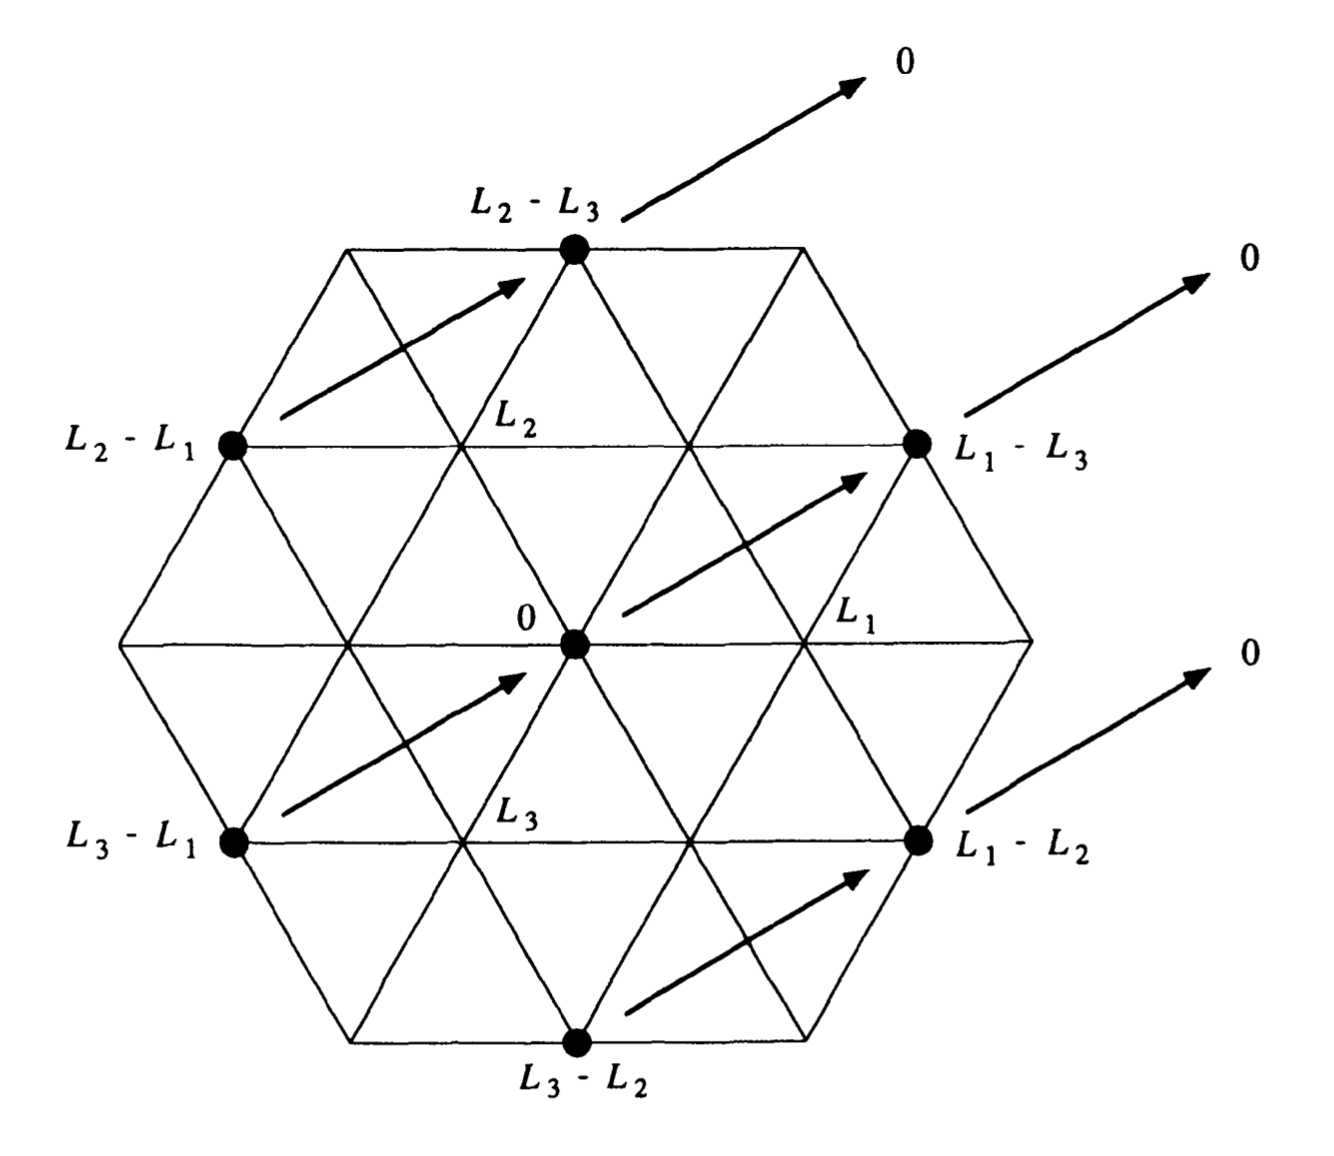
\includegraphics[scale=.3]{L1-L3.png}\end{center}
\end{frame}

\begin{frame}{Bibliography}
	\nocite{*}
	\bibliography{ref}
\end{frame}

\end{document}


















